\documentclass{article}

\usepackage{url,amsmath,amssymb,amsthm,inputenc,xcolor,graphicx,float,placeins,afterpage}
\newcommand\tab[1][1cm]{\hspace*{#1}}
\usepackage{amsmath,amssymb,amsthm,inputenc,xcolor}
\newcommand{\red}[1]{\textcolor{red}{[#1]}} %displays red comments
%\newcommand{\red}[1]{}} %doesn't display comments

\title{Undergraduate Research}
\author{Kenneth L. Budzinski}
\date{4/4/17}

\begin{document}

\maketitle
\tableofcontents

\vspace{8mm}
\red{Rough Introduction, Probably going to have to be rewritten and reworked}
\red{Basically wrote it to get a better understanding of all the things I have done so far}
\red{will probably end up doing the introduction last as it is always usually the hardest part for me to write in papers}
\vspace{5mm}
\newpage
\section{Introduction}
For the past 15 weeks I have been working under Dr. Paul Bauman doing undergraduate research. During this time I was able to learn many different skills,programs, and mathematically techniques to help solve different Problems. Over the Winter Break for this year, I worked on learning about the Finite Element Method, and Dr. Bauman's GRINS Program, which is a Multi-Physics Finite Element package, as well as learning just how to navigate and use the linux operating system, and what github was. By the end of the winter break I was able to formulate my very own Weak from of a 1-d Isobaric Premixed laminar flame problem. For the past 7 weeks I have been working on getting to know the GRINS Framework and learning Paraview to view and understand what was going on in some of the different GRINS examples. I also started learning Latex to write things like this. Since then I have been working on modifying one of the examples to run and model Methane combustion. Alot has gone in along with this, like learning about the GRI30 model for methane combustion, as well as the different types of NASA Glenn Coefficients( 7 coefficients and 9 coefficients) and how they are used to calculate diferent Thermodynamic properties of individual chemical species. The lack of NASA 9 coefficients for a couple of species incorporated in the Methane combustion required an update to the antioch program that is used withing Grins to solve the reactions in Methane Combustion to incorporate NASA 7, During this I helped by making a file containing all of the species in Methane combustion and their NASA 7 coefficients, which were all obtained from GRI30 Thermodynamic data. This file was effentially then pulled and incorporated into the actual Antioch framework as a default file for NASA7. Along with this I had to obtain an xml file with the kinetics data as well as edit the default antioch chemical mixture data file to include the standard enthalpy of formation at 0 k for 5 or so species, which were obtained from atct.anl.gov/Thermochemical Data/version 1.118/species.






















\vspace{5mm}
\red{This is the start of my Weak form formulation where i spent most of the Winter Break learning basic Finite Element Method to accomplish}\\
\vspace{5mm}
\red{Still Need to add all of my references into this section}\\
\newpage
\section{Weak Form of a One-Dimensional Isobaric Premixed Laminar Flame}

After neglecting viscous effects, body forces, radioactive heat transfer, and the diffusion of heat due to concentration gradiants, we are able to reduce the three-dimensional governing equations quite dramatically into a set of one-dimensional differential equations.





\subsection{Boundary Conditions}
The boundary conditions for our one-dimensional premixed laminar flame contain information from the reactant stream and the hot stream. The Reactant stream boundary conditions are:
\begin{align}
  T(-\infty) &= T_{u} \\
  Y_{k}(-\infty) &= \epsilon_{k}({\phi}), \quad k=1,..,N_{sp}
  \end{align}
Here $T_{u}$ is just the cold reactant stream temperature and $\epsilon_{k}(\phi)$ is the known incoming mass flux fraction of the kth species which depends on the reactant stream equivalaence ratio $\phi$. In the hot stream:
\begin{align}
  T'(\infty) & = 0\\
  Y_{k}`(\infty) &= 0,\quad k=1,..,N_{sp}
\end{align}
We also impose a temperature at the origin:
\begin{equation}
  T(0) = T_{i}
\end{equation}
Here the I apply the use of ' to signify a differentiation in x. We then choose a length L which is large enough to ensure vanishingly small derivatives above this length to decrease our space to ($-\infty,0$] and instead replace the Boundary conditions with:
\begin{align}
  T'(L) & = 0\\
  Y_{k}`(L) &= 0, \quad k=1,..,N_{sp}
\end{align}
To eliminate the interval between ($-\infty,0$) we can integrate the species conservation equation between this interval and assume that $T_{i}$ is small enough that the production terms for the species are negligable for T$\leq T_{i}$, we then obtain mixed boundary conditions for the species at the origin:
  \begin{equation}
\dot{M}Y_{k}(0) +\rho(0)Y_{k}(0)u_{k}(0) = \dot{M}\epsilon_{k}(\phi), \quad k=1,..,N_{sp}
  \end{equation}
  Using Fick's law with mixture-averaged diffusion coefficients, we are able to remove the species diffusion velocities from the equation:
  \begin{equation}
    Y_{k}\textbf{u}_{k} = -D_{km}\nabla Y_{k}\\
  \end{equation}
  Here $-D_{km}$ is the effective average diffusion coefficient of species k into the mixture. After substituting for the species diffusion velocities and solving for $Y_{k}$' we obtain:
  \begin{equation}
    Y_{k}' = \frac{\dot{M}(Y_{k}(0)-\epsilon_{k}(\phi)}{\rho(0)D_{km}}
  \end{equation}
  If we integrate the enthalpy conservation equation between $-\infty$ and 0 we obtain:
  \begin{align}
    \dot{M}\big(&\sum_{k=1}^{N_{sp}}Y_{k}(0)u_{k}(0)h_{k}(T(0))-\sum_{k=1}^{N_{sp}}\epsilon(\phi)h_{k}(T_{u})\big) \nonumber \\
    & +\rho(0)\sum_{k=1}^{N_{sp}}Y_{k}(0)u_{k}h_{k}(T(0))-\lambda (0)T'(0) = 0
  \end{align}
  which when combined with (5) and (8) give for the boundary condition for T'(0):
  \begin{equation}
    T'(0) = \frac{\dot{M}}{\lambda(0)}\sum_{k=q}^{N{sp}}\epsilon_{k}(\phi)(h_{k}(T(0))-h_{k}(T_{u}))
    \end{equation}
    We now have boundary conditions for T' and $Y_{k}$' on the space [0,L]






  \subsection{Conservation of energy equation}
The conservation of energy equation for a one-dimensional premixed laminar flame reduces down to:
\begin{equation}
  c_{p}\dot{M}T' = (\lambda T')'-\sum_{k=1}^{N_{sp}} \rho Y_{k}u_{k}c_{p,k}T'-\sum_{k=1}^{N_{sp}}\dot{w_{k}}h_{k}W_{k}
\end{equation}
   Inserting Fick's law into the energy equation we obtain:
  \begin{equation}
    c_{p}\dot{M}T' = (\lambda T')'+\sum_{k=1}^{N_{sp}} \rho D_{km} Y'_{k}c_{p,k}T'-\sum_{k=1}^{N_{sp}}\dot{w_{k}}h_{k}W_{k}
  \end{equation}
  To then obtain the weak form of this equation we integrate over our whole space and multiply by a test function $\sigma$ :
 
  \begin{equation}
   \int_{0}^{L}[c_{p}\dot{M}T'\sigma-(\lambda T')'\sigma-\sum_{k=1}^{N_{sp}} \rho D_{km}Y_{k}'c_{p,k}T'\sigma+\sum_{k=1}^{N_{sp}}\dot{w_{k}}h_{k}W_{k}\sigma] dx = 0 \\
  \end{equation}
  We then use integration by parts and insert our boundary conditions to obtain:
  
    \begin{align}
      \int_{0}^{L}[c_{p}\dot{M}T'\sigma+\lambda T'\sigma '-\sum_{k=1}^{N_{sp}}&\rho D_{km}Y_{k}'c_{p,k}T'\sigma+\sum_{k=1}^{N_{sp}}\dot{w_{k}}h_{k}W_{k}\sigma ]dx \nonumber \\
      + \sigma(0)\dot{M}\sum_{k=1}^{N_{sp}}\epsilon _{k}(\phi)&(h_{k}(T(0))-h_{k}(T_{u})) = 0
    \end{align}


    \subsection{Species Mass Equation}
    The Balancing of the individual species mass for the premixed laminar flame in one dimenstion boils down to, after application of Fick's law once again:
    \begin{equation}
      \dot{M}Y_{k}' = (\rho Y_{k}'D_{km})'+\dot{w_{k}}W_{k},\quad k=1,..,N_{sp}
    \end{equation}
    We then multiply by our test function $\gamma_{k}$ and integrate over our whole space to obtain a weak form of the equation:
    \begin{equation}
      \int_{0}^{L}[\dot{M}Y_{k}'\gamma_{k}-(\rho Y_{k}'D_{km})'\gamma_{k}-\dot{w_{k}}W_{k}\gamma_{k}]dx = 0,\quad k=1,..,N_{sp}
    \end{equation}
    once again we integrate by parts and apply our boundary conditions to obtain:
    \begin{equation}
      \int_{0}^{L}[\dot{M}Y_{k}'\gamma_{k}+(\rho Y_{k}'D_{km})\gamma_{k}'-\dot{w_{k}}W_{k}\gamma_{k}]dx + \dot{M}(Y_{k}(0)-\epsilon_{k}(\phi))\gamma_{k} = 0,\quad k=1,..,N_{sp}
      \end{equation}




    \subsection{Conservation of Mass Equation}
    The Conservation of the total mass in the system allows us to conclude that for the whole system:
    \begin{equation}
    \dot{M} = \rho u = \text{constant}
\end{equation}
to convert this into a weak form equation we can just use the method of lagrange multipliers and multiply our residual by the scalar test function $\psi$
\begin{equation}
  \psi(\dot{M}-\rho u) = 0
\end{equation}

\subsection{Other Constraint equation}
Along with the conservation of Mass equation, we also include the ideal gas law to constrain our system of equations:
\begin{equation}
  \rho = \frac{P\bar{W}}{RT}
\end{equation}






\subsection{Weak statement form of our problem}
  Overall, the weak statement of our problem is to find a \textbf{u}=($T,Y_{k},\dot{M}$) and a \textbf{v}=($\sigma,\gamma,\psi$) that is a solution to
  \begin{align*}
    \int_{0}^{L}[c_{p}\dot{M}T'\sigma&+\lambda T'\sigma '-\sum_{k=1}^{N_{sp}}\rho D_{km}Y_{k}'c_{p,k}T'\sigma+\sum_{k=1}^{N_{sp}}\dot{w_{k}}h_{k}W_{k}\sigma ]dx  \\
    &+ \sigma(0)\dot{M}\sum_{k=1}^{N_{sp}}\epsilon _{k}(\phi)(h_{k}(T(0))-h_{k}(T_{u})) = 0 \\
    \int_{0}^{L}[\dot{M}Y_{k}'\gamma_{k}&+(\rho Y_{k}'D_{km})\gamma_{k}'-\dot{w_{k}}W_{k}\gamma_{k}]dx + \dot{M}(Y_{k}(0)-\epsilon_{k}(\phi))\gamma_{k} = 0,\quad k=1,..,N_{sp} \\
   &\qquad \psi(\dot{M}-\rho u) = 0 \\
    &\qquad\rho = \frac{P\bar{W}}{RT} 
    \end{align*}






\newpage
\section{GRI3.0 Modeling with Grins}
\tab Using GRINS, a Multiphysics finite element package built on libmesh, I was tesked with modeling the GRI-Mech 3.0 mechanism that models natural gas combustion, NO formation, and reburn chemistry.\red{Maybe add a section about GRINS \& ANtioch Here} The GRI mechanism contains 53 species and over \red{find actual number} 325 Reactions, Using the species data and thermodynamic data supplied by the mechanism I was able to run a 2-d example using GRINS. However, one of the first problems I ran into doing this was the lack of support GRINS had for NASA-7 coefficients, which was the format of the thermodynamic data supplied by GRI-3.0.
\red{Add that the Nasa coefficients are fits for enthalpy,entropy, and standard heat capacity at constant pressure}
\subsection{Nasa 9 \& Nasa 7 Comparison}
\tab  Since Grins was only developed to parse Nasa 9 data, I had to try and find the NASA 9 data from the Nasa website itself. Some species used in the GRI-3.0 Mechanism could not be found there however, so I needed to convert the Nasa 7 species data obtained from the GRI-Mech 3.0 into a Nasa 9 form. To do this I studied how each form was fit.

\subsubsection{Nasa Coefficients}
\tab Nasa Lewis-Glenn Coefficients, or Nasa coefficients for short, are the coefficients of a universal fitting method used for calculating the thermodynamic properties of different species at different temperatures. Storing these thermodynamic data in the form of empirical equations  allow for analytical integrations and condenses all the information on the species into just a few constants that can reproduce these data points. These coefficients were first used in 1971, where the Nasa 7 composition of these coefficients were conceptualized. This original format used 7 coefficients to caclulate the $\frac{C_p}{R}$, $\frac{H}{RT}$, $\frac{S}{R}$ as a function of temperature from a range of 300 to up to 5000K. These Nasa 7 equations are:
\begin{align*}
 \frac{C_P}{R} =&  a_0+a_1T + a_2T^2 + a_3T^3 + a_4T^4\\
 \frac{H}{RT}  =&  a_0 + a_1\frac{T}{2} + a_2\frac{T^2}{3} + a_3\frac{T^3}{4} + a_4\frac{T^4}{5} + \frac{a_5}{T}\\
 \frac{S}{R} =&   a_0ln{T} + a_1T + a_2\frac{T^{2}}{2} + a_3\frac{T^3}{3} + a_4\frac{T^4}{4} + a_6\\
\end{align*}
Around the turn of the century, the method used in forming these coefficients was altered to adapt two additional terms in the curve fitting of the thermodynamic data. This new format of the coefficients is appropriately called  'Nasa 9 coefficients'. The two new additional terms are coefficients associated with the new $T^{-1}$ and $T^2$ terms added to the $C_p$ fits. The format wasn't only selected to accomodate these two constants but also allows for future revisions and expansions in the future. It allows for variable temperature intervals, and is easier to read. The format acutally uses 10 coefficients, however the 8th coefficient is always set 0, this helps in making them easier to read. The Thermodynamic equations resulting from these coefficients for Nasa 9 are:
\begin{align*}  
  \frac{C_P}{R} = \quad &a_0T^{-2} + a_1T^{-1} + a_2+a_3T + a_4T^2 + a_5T^3 + a_6T^4\\
  \frac{H}{RT} = -&a_0t^{-2} + a_1\frac{ln{T}}{T} + a_2 + a_3\frac{T}{2} + a_4\frac{T^2}{3} + a_5\frac{T^3}{4} + a_6\frac{T^4}{5} + \frac{a_8}{T}\\
  \frac{S}{R} =  -&a_0\frac{T^{-2}}{2} - a_1T^{-1} + a_2ln{T} + a_3T + a_4\frac{T^{2}}{2} + a_5\frac{T^3}{3} + a_6\frac{T^4}{4} + a_9\\
\end{align*}
As we see, the Nasa 7 format can be transformed into the Nasa 9 format by setting the added coefficients to 0 and moving the 7 formats coefficients to match their positions in the new format. When we do this, we have to remember the different temperature ranges these formats span. 
\subsubsection{Nasa 7 vs Nasa 9}
To make sure that the changing of the format didn't alter the thermodynamic properties obtained from the coefficients to much, I analyzed a couple species that had both types of coefficients available. I studied them plotted together at different temperatures as well as the linear interpolation of Nasa 7 after it reached its max temperature range agains the Nasa 9 fits. The plots were obtained for the species HCO and are plotted below:
\red{Better align Graphs}


\begin{figure}[!bp]
  \centering
  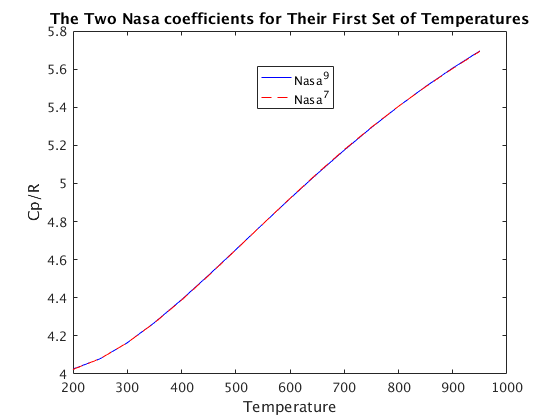
\includegraphics[width=.8\linewidth]{./NasaPlots/Cp1.png}
  \label{fig:cp1}
  \caption{HCO comparison of Nasa 7 vs Nasa 9 data}
\end{figure}



\begin{figure}[!p]
  \centering
  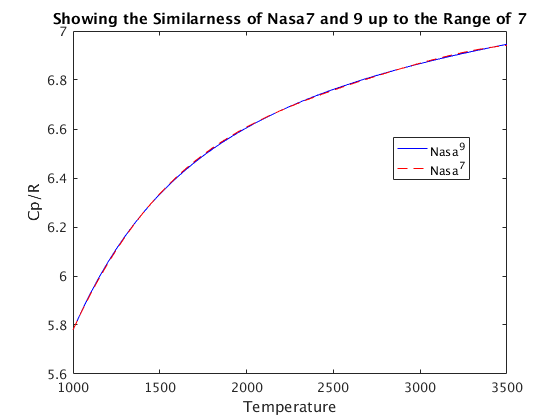
\includegraphics[width=.8\linewidth]{./NasaPlots/Cp2.png}
  \label{fig:cp2}
  \caption{HCO comparison of Nasa 7 vs Nasa 9 data}
\end{figure}


\begin{figure}[!p]
  \centering
  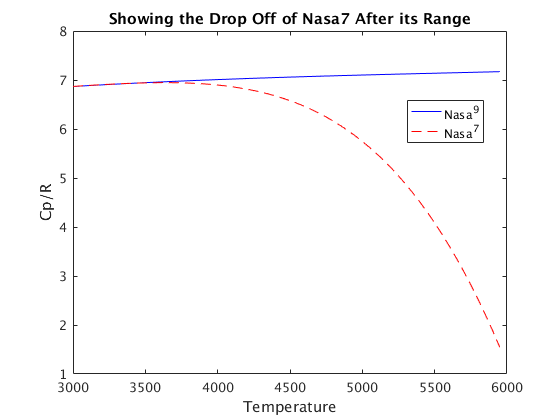
\includegraphics[width=.8\linewidth]{./NasaPlots/Cp3.png}
  \label{fig:cp3}
  \caption{HCO comparison of Nasa 7 vs Nasa 9 data}
\end{figure}

 \begin{figure}[!p]
  \centering
  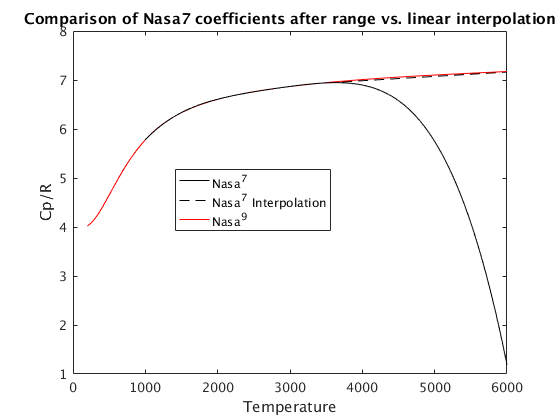
\includegraphics[width=.8\linewidth]{./NasaPlots/CpT.png}
  \label{fig:cpT}
  \caption{HCO comparison of Nasa 7 vs Nasa 9 data, along with linearly interpolated data for data outside of Nasa 7's range for $\frac{C_p}{R}$ data}
\end{figure}

\begin{figure}[!p]
  \centering
  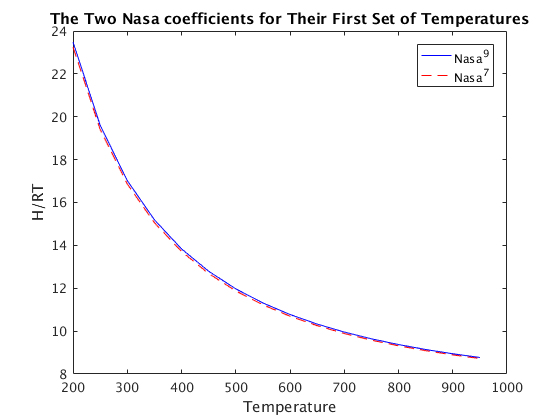
\includegraphics[width=.8\linewidth]{./NasaPlots/H1.png}
  \label{fig:H1}
  \caption{HCO comparison of Nasa 7 vs Nasa 9 data}
\end{figure}


\begin{figure}[!p]
  \centering
  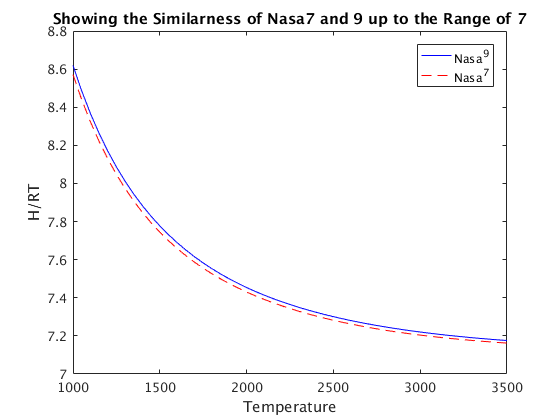
\includegraphics[width=.8\linewidth]{./NasaPlots/H2.png}
  \label{fig:H2}
  \caption{HCO comparison of Nasa 7 vs Nasa 9 data}
\end{figure}


\begin{figure}[!p]
  \centering
  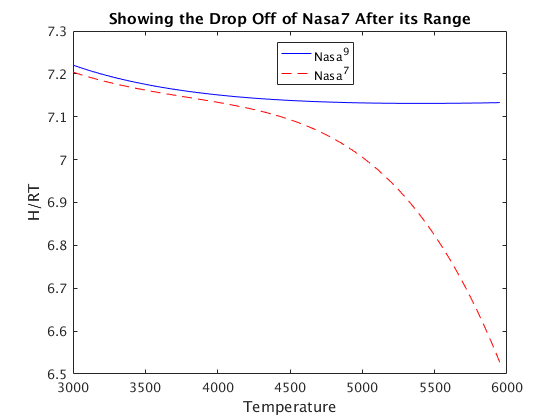
\includegraphics[width=.8\linewidth]{./NasaPlots/H3.png}
  \label{fig:H3}
  \caption{HCO comparison of Nasa 7 vs Nasa 9 data}
\end{figure}

\begin{figure}[!p]
  \centering
  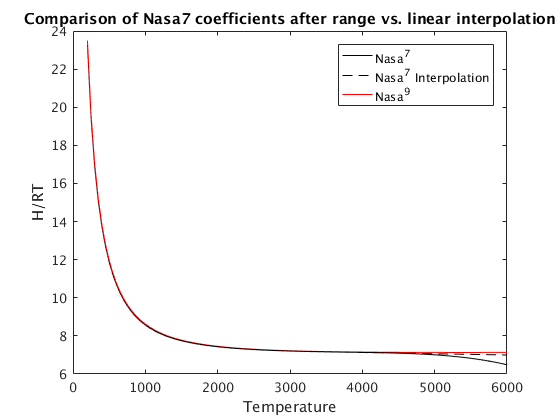
\includegraphics[width=.8\linewidth]{./NasaPlots/HT.png}
  \label{fig:HT}
  \caption{HCO comparison of Nasa 7 vs Nasa 9 data, along with linearly interpolated data for data outside of Nasa 7's range for $\frac{H}{RT}$ data}
\end{figure}


\begin{figure}[!p]
  \centering
  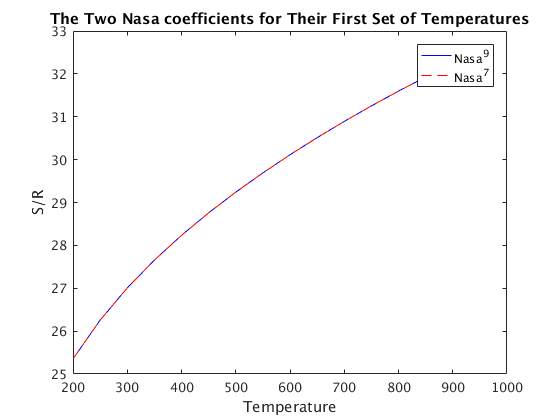
\includegraphics[width=.8\linewidth]{./NasaPlots/S1.png}
  \label{fig:s1}
  \caption{HCO comparison of Nasa 7 vs Nasa 9 data}
\end{figure}


\begin{figure}[!p]
  \centering
  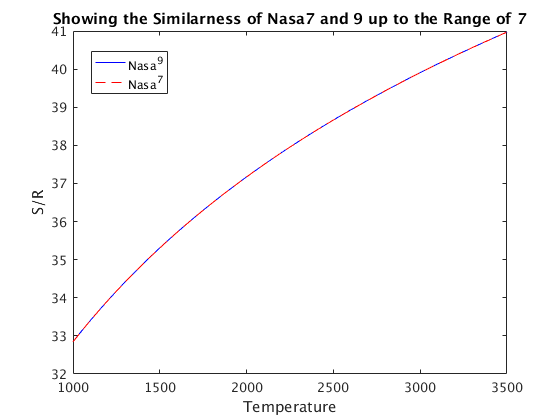
\includegraphics[width=.8\linewidth]{./NasaPlots/S2.png}
  \label{fig:S2}
  \caption{HCO comparison of Nasa 7 vs Nasa 9 data}
\end{figure}


\begin{figure}[!p]
  \centering
  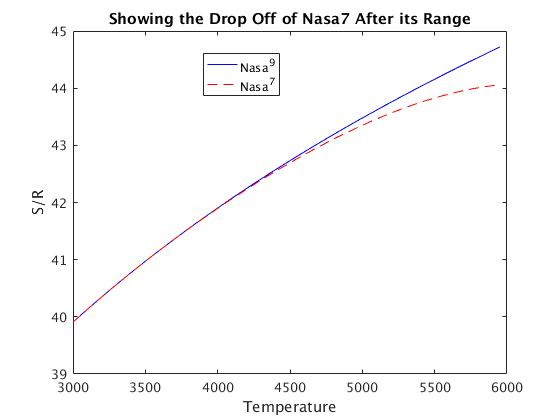
\includegraphics[width=.8\linewidth]{./NasaPlots/S3.png}
  \label{fig:S3}
  \caption{HCO comparison of Nasa 7 vs Nasa 9 data}
\end{figure}

\begin{figure}
  \centering
  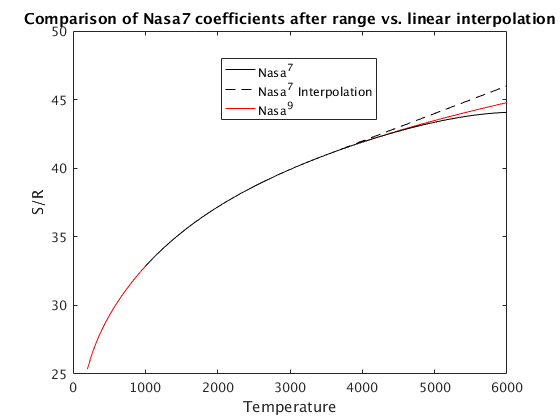
\includegraphics[width=.8\linewidth]{./NasaPlots/ST.png}
  \label{fig:sT}
  \caption{HCO comparison of Nasa 7 vs Nasa 9 data, along with linearly interpolated data for data outside of Nasa 7's range for $\frac{S}{R}$ data}
\end{figure}

\newpage


%Starting Bibliography
\bibliographystyle{plain}
\bibliography{CEAS,NASAbib}


\nocite{*}

\end{document}





